% !TEX root = ../main.tex

%\newpage
\section{Policy and Screenshot for Twitter}
\label{app:twitter-sources}

Section~\ref{app:twitter-abusive-behavior} documents Twitter's policy on abusive
behavior as of 5 September, 2022. It preserves the structure and formatting of
the original, with links pointing to the Internet Archive. The current version
of the policy is available at
\url{https://help.twitter.com/en/rules-and-policies/abusive-behavior}.
Section~\ref{app:twitter-staging} documents Twitter's user interface for a
locked account with the violative tweet at the center.


\subsection{Abusive Behavior}
\label{app:twitter-abusive-behavior}

\noindent\href{https://web.archive.org/web/20220905021323/https://help.twitter.com/en/rules-and-policies/twitter-rules.html}{Twitter
Rules}: You may not engage in the targeted harassment of someone, or incite
other people to do so. We consider abusive behavior an attempt to harass,
intimidate, or silence someone else's voice.


\subsubsection{Rationale}

On Twitter, you should feel safe expressing your unique point of view. We
believe in freedom of expression and open dialogue, but that means little as an
underlying philosophy if voices are silenced because people are afraid to speak
up.

In order to facilitate healthy dialogue on the platform, and empower individuals
to express diverse opinions and beliefs, we prohibit behavior that harasses or
intimidates, or is otherwise intended to shame or degrade others. In addition to
posing risks to people's safety, abusive behavior may also lead to physical and
emotional hardship for those affected.

Learn more about our approach to
\href{https://web.archive.org/web/20220905021323/https://help.twitter.com/en/rules-and-policies/enforcement-philosophy.html}{policy
development and our enforcement philosophy}.


\subsubsection{When This Applies}

Some Tweets may seem to be abusive when viewed in isolation, but may not be when
viewed in the context of a larger conversation. When we review this type of
content, it may not be clear whether it is intended to harass an individual, or
if it is part of a consensual conversation. To help our teams understand the
context of a conversation, we may need to hear directly from the person being
targeted, to ensure that we have the information needed prior to taking any
enforcement action.

We will review and take action against reports of accounts targeting an
individual or group of people with any of the following behavior within Tweets
or Direct Messages. For accounts engaging in abusive behavior on their profile,
please refer to our
\href{https://web.archive.org/web/20220905021323/https://help.twitter.com/en/rules-and-policies/abusive-profile.html}{abusive
profile policy}. For behavior targeting people based on their race, ethnicity,
national origin, sexual orientation, gender, gender identity, religious
affiliation, age, disability, or serious disease, this may be in violation of
our
\href{https://web.archive.org/web/20220905021323/https://help.twitter.com/en/rules-and-policies/hateful-conduct-policy.html}{hateful
conduct policy}.

\begin{description}

\item[Violent Threats] \hfill

    We prohibit content that makes violent threats against an identifiable
    target. Violent threats are declarative statements of intent to inflict
    injuries that would result in serious and lasting bodily harm, where an
    individual could die or be significantly injured, e.g., ``I will kill you.''

    \textbf{Note}: We have a zero tolerance policy against violent threats.
    Those deemed to be sharing violent threats will face immediate and permanent
    suspension of their account.

\item[Wishing, hoping, or calling for serious harm on a person or group of
    people] \hfill

    We do not tolerate content that wishes, hopes, promotes, incites, or
    expresses a desire for death, serious bodily harm or serious disease against
    an individual or group of people. This includes, but is not limited to:

    \begin{itemize}
    \item Hoping that someone dies as a result of a serious disease e.g., ``I
        hope you get cancer and die.''
    \item Wishing for someone to fall victim to a serious accident e.g., ``I
        wish that you would get run over by a car next time you run your
        mouth.''
    \item Saying that a group of individuals deserves serious physical injury
        e.g., ``If this group of protesters don't shut up, they deserve to be
        shot.''
    \end{itemize}

\item[About wishes of harm exceptions on Twitter] \hfill

    We recognize that conversations regarding certain individuals credibly
    accused of severe violence may prompt outrage and associated wishes of harm.
    In these limited cases, we will request the user to delete the Tweet without
    any risk of account penalty, strike, or suspension. Examples are, but not
    limited to:

    \begin{itemize}
    \item ``I wish all rapists to die.''
    \item ``Child abusers should be hanged.''
    \end{itemize}

\item[Unwanted sexual advances] \hfill

    While some
    \href{https://web.archive.org/web/20220905021323/https://help.twitter.com/en/rules-and-policies/media-policy.html}{consensual
    nudity and adult content is permitted} on Twitter, we prohibit unwanted
    sexual advances and content that sexually objectifies an individual without
    their consent. This includes, but is not limited to:

    \begin{itemize}
    \item sending someone unsolicited and/or unwanted adult media, including
        images, videos, and GIFs;
    \item unwanted sexual discussion of someone's body;
    \item solicitation of sexual acts; and
    \item any other content that otherwise sexualizes an individual without
        their consent.
    \end{itemize}

\item[Using insults, profanity, or slurs with the purpose of harassing or
    intimidating others] \hfill

    We take action against the use of insults, profanity, or slurs to target
    others. In some cases, such as (but not limited to) severe, repetitive usage
    of insults or slurs where the primary intent is to harass or intimidate
    others, we may require Tweet removal. In other cases, such as (but not
    limited to) moderate, isolated usage of insults and profanity where the
    primary intent is to harass or intimidate others, we may limit Tweet
    visibility as further described below. Please also note that while some
    individuals may find certain terms to be offensive, we will not take action
    against every instance where insulting terms are used.

\item[Encouraging or calling for others to harass an individual or group of
    people] \hfill

    We prohibit behavior that encourages others to harass or target specific
    individuals or groups with abusive behavior. This includes, but is not
    limited to; calls to target people with abuse or harassment online and
    behavior that urges offline action such as physical harassment.

\item[Denying mass casualty events took place] \hfill

    We prohibit content that denies that mass murder or other mass casualty
    events took place, where we can verify that the event occured [sic], and

    when the content is shared with abusive intent. This may include references
    to such an event as a ``hoax'' or claims that victims or survivors are fake
    or ``actors.'' It includes, but is not limited to, events like the
    Holocaust, school shootings, terrorist attacks, and natural disasters.

\item[Do I need to be the target of this content for it to be reviewed for
    violating the Twitter Rules?] \hfill

    No, we review both first-person and bystander reports of such content.
\end{description}


\subsubsection{Consequences}

When determining the penalty for violating this policy, we consider a number of
factors including, but not limited to, the severity of the violation and an
individual's previous record of rule violations. The following is a list of
potential enforcement options for content that violates this policy:
\begin{itemize}
\item Downranking Tweets in replies, except when the user follows the Tweet
    author.
\item Making Tweets ineligible for amplification in Top search results and/or on
    timelines for users who don't follow the Tweet author.
\item Excluding Tweets and/or accounts in email or in-product recommendations.
\item Requiring Tweet removal.
    \begin{itemize}
    \item For example, we may ask someone to remove the violating content and
        serve a period of time in read-only mode before they can Tweet again.
        Subsequent violations will lead to longer read- only periods and may
        eventually result in permanent suspension.
    \end{itemize}
\item Suspending accounts whose primary use we've determined is to engage in
    abusive behavior as defined in this policy, or who have shared violent
    threats.
\end{itemize}
Learn more about
\href{https://web.archive.org/web/20220905021323/https://help.twitter.com/en/rules-and-policies/enforcement-options.html}{our
range of enforcement options}.

If someone believes their account was suspended in error, they can
\href{https://web.archive.org/web/20220905021323/https://help.twitter.com/forms/general?subtopic=suspended}{submit
an appeal}.


\subsection{Twitter's Restricted UI}
\label{app:twitter-staging}

\begin{figure}
\centering
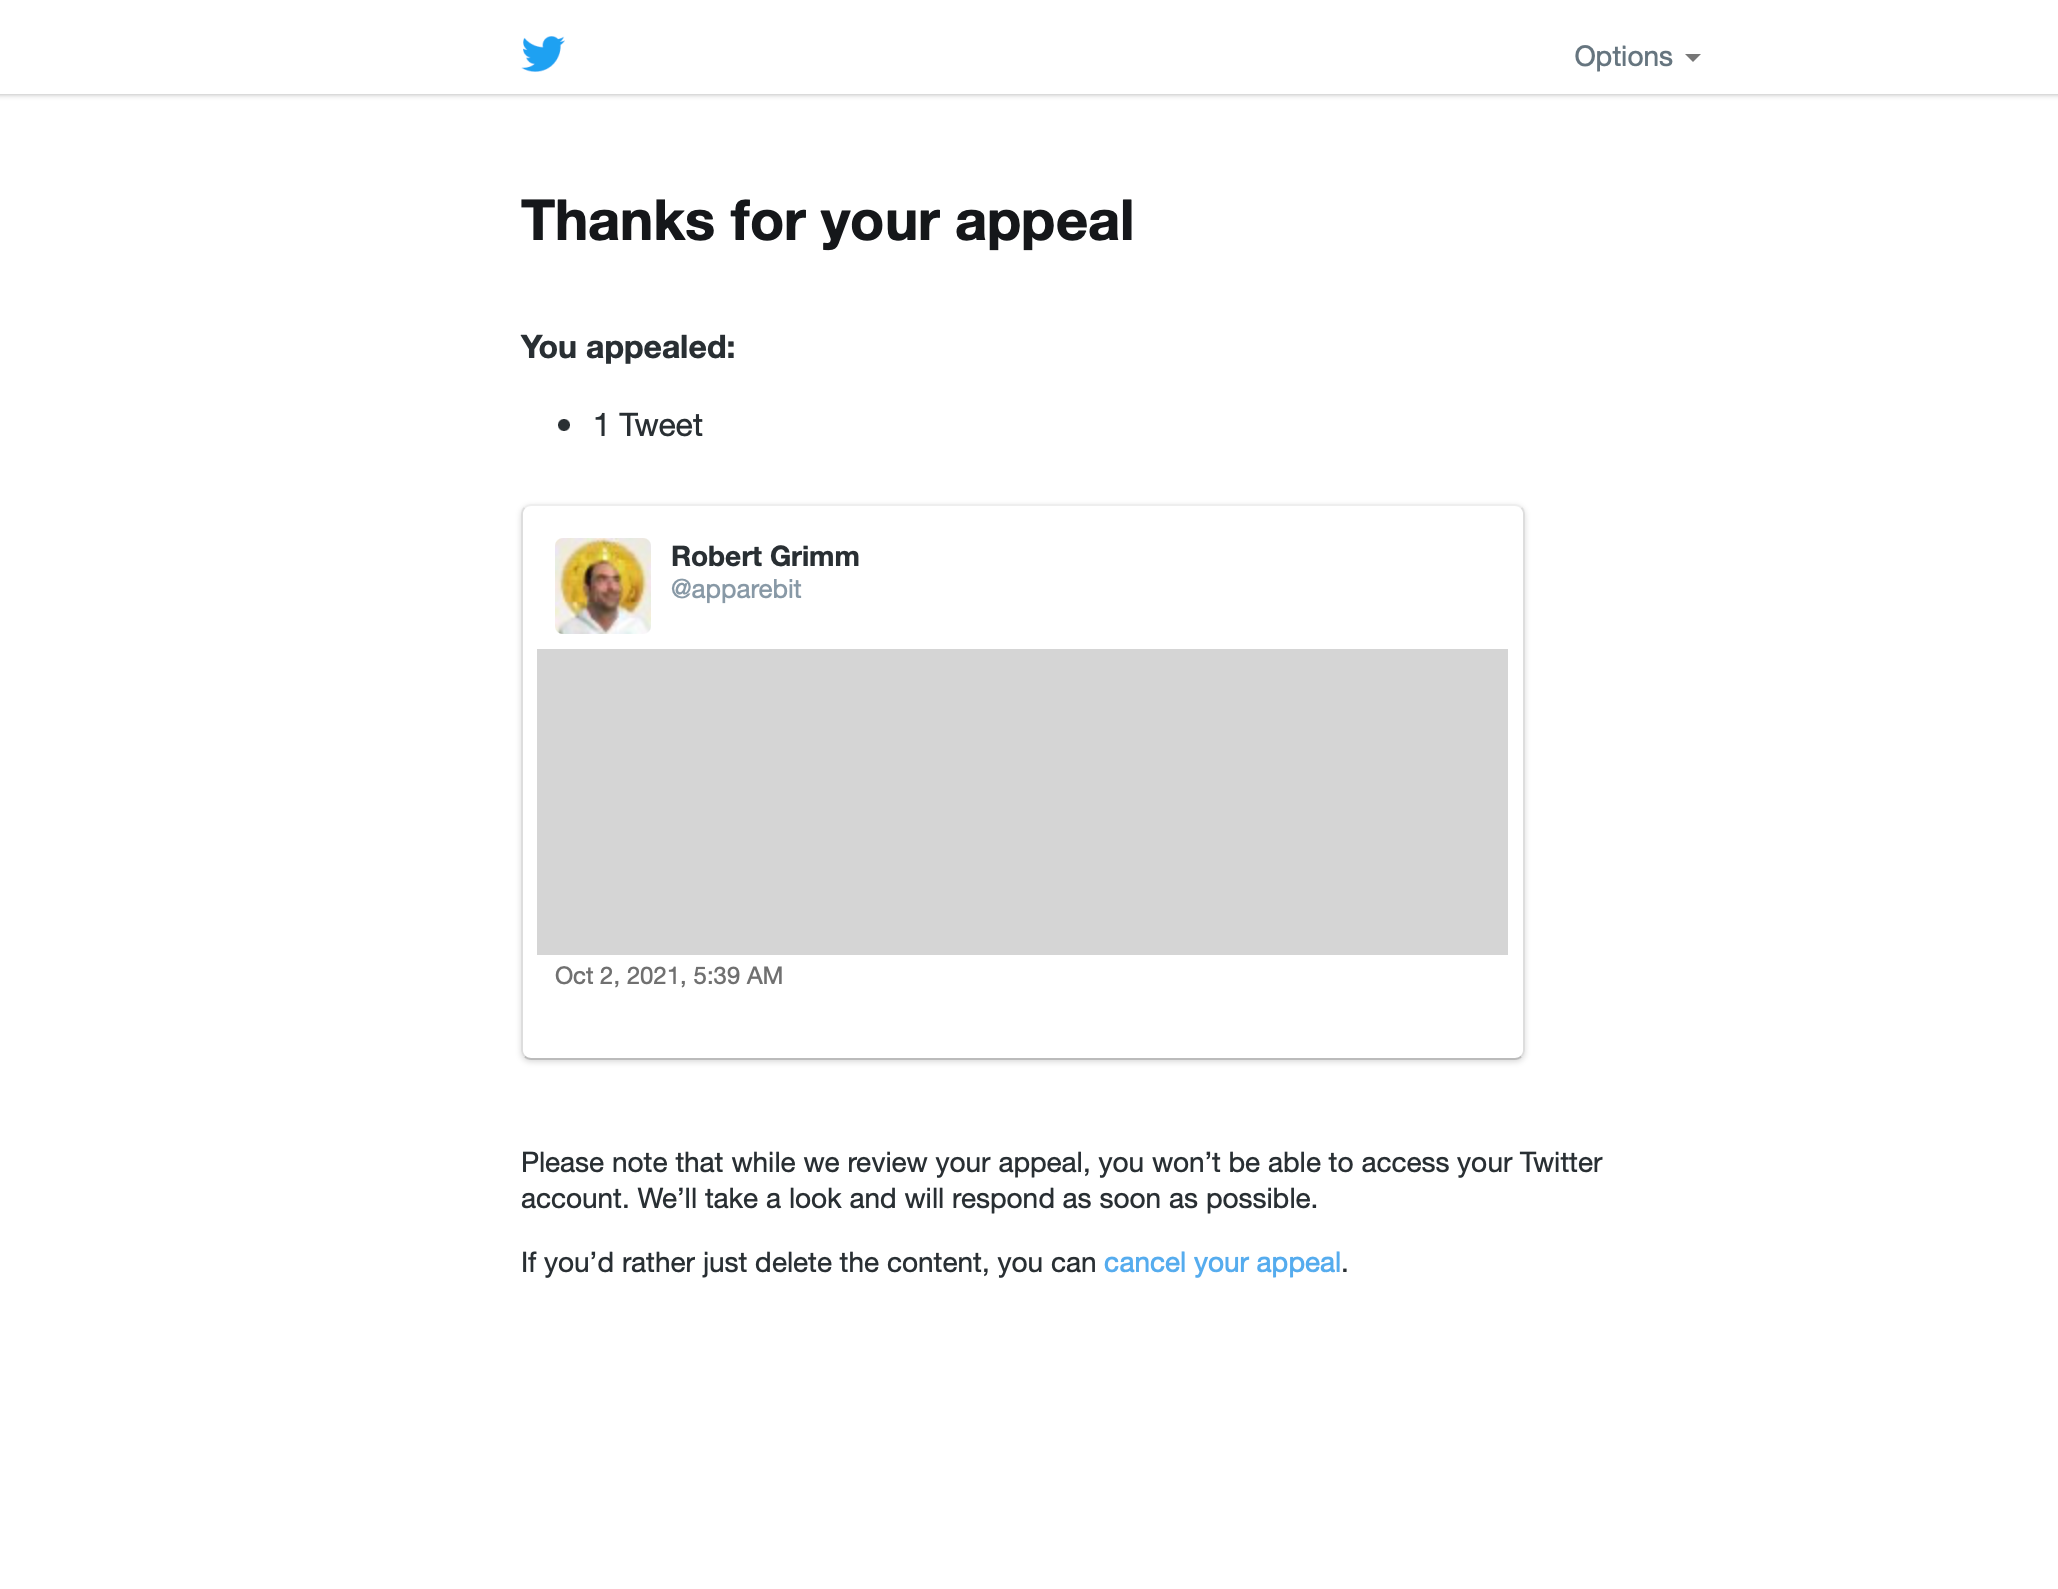
\includegraphics[width=\textwidth]{the-tweet}
\Description{Screenshot showing the violative tweet in the center under the
    headline ``Thanks for your appeal.''}
\caption{Twitter puts the reason for the account being locked right in the center.}
\label{fig:thetweet}
\end{figure}

Figure~\ref{fig:thetweet} shows Twitter's user interface while the account is
locked down. Even after cancelling the appeal but before agreeing to delete the
tweet, the overall structure of the user interface remains but the text above
and below the tweet changes. Twitter's original instructions claimed that
``while in this state, you can still browse Twitter, but you're limited to only
sending Direct Messages to your followers --- no Tweets, Retweets, Fleets,
follows, or likes.'' In reality, none of that is possible while an appeal is
pending. I censored the text of the tweet because of its very incivility.
